\documentclass[12 pt]{article}
%%%%%%%%%%%%%%%%%%%%%%%%%%%%
%\topmargin 0.2in
%\textheight 10in
%\voffset -1.25in
%\textwidth 6.2in
%\parindent 0.25in
%\itemindent 0.in
%\leftmargin 0.5in
%\hoffset -0.8in

%\addtolength{\textwidth}{ain}
%\addtolength{\hoffset}{-bin}
%\addtolength{\textheight}{cin}
%\addtolength{\voffset}{cin}
%a=2b

\addtolength{\textwidth}{1.in}
\addtolength{\hoffset}{-.5in}
\addtolength{\textheight}{1.in}
\addtolength{\voffset}{-1.in}


%Packages
\usepackage{graphicx}
\usepackage[mathcal,mathscr]{eucal}
\usepackage{amsfonts}
\usepackage{mathrsfs}
\usepackage{amsmath, amsthm, amssymb,epsfig,amscd,multicol}
\usepackage{enumitem}
\usepackage{xcolor}
\usepackage{tikz}
%\usetikzlibrary{cd}
\usetikzlibrary{arrows}
\usepackage{float}
\usepackage{caption}
\usepackage{subcaption}
\usepackage{tabu}
\usepackage{xfrac}
\usepackage{arydshln}

%\usepackage{mathptmx}

%New Commands
\newcommand{\R}{\mathbb{R}}
\newcommand{\U}{\mathcal{U}}
\newcommand{\Z}{\mathbb{Z}}
\newcommand{\N}{\mathbb{N}}
\newcommand{\Q}{\mathbb{Q}}
\newcommand{\Ra}{\Rightarrow}
\newcommand{\set}[1]{\left\{#1\right\}}
\newcommand{\ds}{\displaystyle}
\newcommand{\divides}{\! \mid \!}
\newcommand{\ndivides}{\! \nmid \!}
\newcommand{\mymod}[1]{ \ (\bmod \ #1)}

\theoremstyle{definition}
\newtheorem{remark}{Remark}

\theoremstyle{plain}

\newtheoremstyle{mytheorem}% name of the style to be used
  {12pt}% measure of space to leave above the theorem. E.g.: 3pt
  {12pt}% measure of space to leave below the theorem. E.g.: 3pt
  {\itshape}% name of font to use in the body of the theorem
  {0pt}% measure of space to indent
  {\bfseries}% name of head font
  {.}% punctuation between head and body
  {5 pt plus 1pt minus 1pt}% space after theorem head; " " = normal interword space
  {}% Manually specify head
  
 	\theoremstyle{mytheorem}
  	\newtheorem{theorem}{Theorem}[section]%[numbering]
	\newtheorem{lemma}{Lemma}[section]
	\newtheorem{cor}{Corollary}[section]
	

\newtheoremstyle{myexample}% name of the style to be used
  {22pt}% measure of space to leave above the theorem. E.g.: 3pt
  {22pt}% measure of space to leave below the theorem. E.g.: 3pt
  {\normalfont}% name of font to use in the body of the theorem
  {0pt}% measure of space to indent
  {\bfseries}% name of head font
  {.}% punctuation between head and body
  {5 pt plus 1pt minus 1pt}% space after theorem head; " " = normal interword space
  {}% Manually specify head

	\theoremstyle{myexample}
	\newtheorem{example}{Example}[section]
	\newtheorem{claim}{Claim}
	
\newtheoremstyle{mydefinition}% name of the style to be used
  {22pt}% measure of space to leave above the theorem. E.g.: 3pt
  {22pt}% measure of space to leave below the theorem. E.g.: 3pt
  {\normalfont}% name of font to use in the body of the theorem
  {0pt}% measure of space to indent
  {\bfseries}% name of head font
  {.}% punctuation between head and body
  {5 pt plus 1pt minus 1pt}% space after theorem head; " " = normal interword space
  {}% Manually specify head

	\theoremstyle{mydefinition}
	\newtheorem{definition}{Definition}
	\newtheorem*{definition*}{Definition}

\begin{document}
\pagenumbering{gobble}
\begin{center}
\textbf{P.11 More on Proof}
\end{center}

Believe it or not, we've actually covered all of the fundamental proof techniques.  Any statement of the form ``If $P$, then $Q$'' can be proved using direct proof, contrapositive proof, or contradiction proof (assuming the statement can be proven at all).  We will devote the remainder of the semester to writing proofs of particular kinds of statements.  Often, we will still employ one of the methods mentioned above, but there are certain expectations and conventions for these types of proofs that we will follow.
\begin{center}
\fbox{\parbox{5.5in}{Goals:
	\begin{itemize}
	\item Write Biconditional Proofs
	\item Prove Existence Theorems
	\end{itemize}
}}
\end{center}
\section{Biconditional Proofs}
\noindent Recall that a biconditional statement has the form $(P \Leftrightarrow Q)$, which is read as ``$P$ if and only if $Q$''.  This is really just short hand for $(P \Rightarrow Q) \wedge (Q \Rightarrow P)$.  To prove a biconditional statement we must prove both $P \Rightarrow Q$ and its converse $Q \Ra P$.  In other words, we have to write two proofs in one.  Generally speaking, the two pieces may require two different proof techniques.  It is very common that $P \Ra Q$ can be done via direct proof, but $Q \Ra P$ requires proof by contrapositive or contradiction.


\begin{enumerate}
\item Follow the steps below to prove the following claim.
\begin{claim} The integer $n$ is even if and only if $n^2$ is even.
\end{claim}
	\begin{enumerate}[label=(\alph*)]
	\item Determine the two conditional statements that comprise the conditional statement in the claim.
	\vspace{1in}
	\item Prove the first conditional statement using any means you find appropriate.
	\vspace{2in}
	\item Prove the second conditional statement using any means you find appropriate.
	\vspace{2in}
	\item Combine the two proofs to prove the biconditional statement.  Yes, I'm requiring that you write out everything again.  Keep the following in mind: (1) the proofs of the two conditional statements must be in separate paragraphs, and (2) the second paragraph should begin with ``Conversely,'' to indicate that you're proving the converse of the first statment.  When we are writing biconditional proofs by hand, we often label the two directions with ``($\Rightarrow$)'' and ``($\Leftarrow$).''  This is usually considered inappropriate in formal proof writing, but it's a good idea while you try to get used to the technique.

	\end{enumerate}
	\newpage
\item Prove the following biconditional statement.
\begin{claim} Suppose $a,r \in \Z$, $n \in \N$, and $0 \leq r <n$.  Then $a \equiv r (\bmod \ n)$ if and only if $a$ has remainder $r$ when divided by $n$.
\end{claim}
\vspace{4in}
\end{enumerate}
\noindent  Other than the fact that you have to write two proofs in one, there's really nothing new to you about writing biconditional proofs.  Therefore, we'll move on to something that is new.

\section{Equivalent Statements}
If the statement ``$P$ if and only if $Q$'' holds, then we often refer to $P$ and $Q$ as equivalent statements.  This is because if we know that one is true then we can automatically assume that the other is also true.  There are many very important theorems in math (especially in linear algebra) that are really just a list of equivalent statements.  The example below gives such a list (this example is not from linear algebra).
\begin{claim}The following statements are equivalent.
	\begin{enumerate}[label=(\alph*)]
	\item The integer $n$ is even.
	\item The integer $n^2$ is even.
	\item The integer $n^3$ is even.
	\item The integer $n^2$ is divisible by 4.
	\end{enumerate}
\end{claim}
Again, by equivalent the claim means the biconditional statements $(a) \Leftrightarrow (b)$, $(a) \Leftrightarrow (c)$, $(b) \Leftrightarrow (c)$, and (c) $\Leftrightarrow$ (d) are all true.  The diagram below shows the relationships between the statements.

\begin{figure}[H]
\centering
\frame{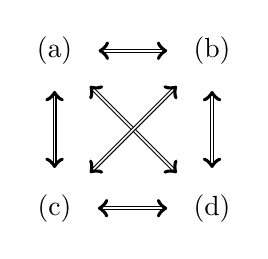
\begin{tikzpicture}[-,shorten <=6pt, shorten >=6pt,auto,node distance=2cm]
\node (a) {(a)};
\node (b) [right of=a] {(b)};
\node (c) [below of =a] {(c)};
\node (d) [below of=b] {(d)};

\path[every node/.style]
(a) edge [double,<->] (b)
	edge [double, <->] (c)
	edge [double, <->] (d)
(b) 	edge [double, <->]  (c)
	edge [double, <->] (d)
(c) edge [double,<->] (d);
\end{tikzpicture}}
\end{figure}

In reality, this diagram is equivalent to the one below.  If we wanted to prove the claim, it would be easiest to prove the relationships as described in the following diagram because it would require fewer proof directions.

\begin{figure}[h]
\centering
\frame{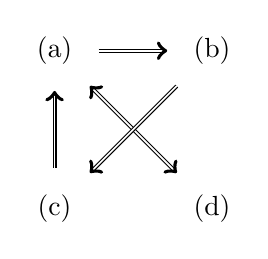
\begin{tikzpicture}[-,shorten <=6pt, shorten >=6pt,auto,node distance=2cm]
\node (a) {(a)};
\node (b) [right of=a] {(b)};
\node (c) [below of =a] {(c)};
\node (d) [below of=b] {(d)};

\path[every node/.style]
(a) edge [double,->] (b)
	edge [double, <-] (c)
	edge [double,<->] (d)
(b) 	edge [double, ->]  (c);
\end{tikzpicture}}
\end{figure}

Unfortunately, proving $(b) \Rightarrow (c)$ would be difficult, so we would have to prove this claim according to the following diagram.  It requires six proof directions, but it's still the easiest way to go.

\begin{figure}[h]
\centering
\frame{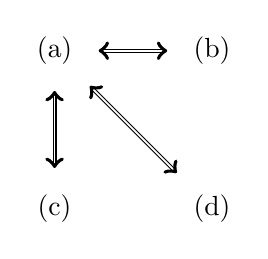
\begin{tikzpicture}[-,shorten <=6pt, shorten >=6pt,auto,node distance=2cm]
\node (a) {(a)};
\node (b) [right of=a] {(b)};
\node (c) [below of =a] {(c)};
\node (d) [below of=b] {(d)};

\path[every node/.style]
(a) edge [double,<->] (b)
	edge [double, <->] (c)
	edge [double, <->] (d);
\end{tikzpicture}}
\end{figure}

We won't actually write any equivalent statement proofs this semester.  They only employ the methods we know, so ultimately they just take longer than the proofs we write otherwise.  Still, you should be aware of them and prepared to see them in future courses.


\section{Existence Proofs}
Thus far we've only proved statements of the form $P \Rightarrow Q$.  Even biconditional statements amount to proving this type of statement.  We move now to proving ``existence'' statements.  Existence statements are statement that claim that some entity exists.  They take the form 
\[ \exists \ x, \ P(x).\]

\noindent Recall that in the above notation, $P$ is a statement whose truth value depends on the value of $x$.  Proving existence statements is actually quite simple in concept.  All we have to do is give an example of the thing that's supposed to exist.  Of course, our proof should also include an explanation of why our example fits the requirements of the claim.

\begin{claim} There exists a smallest odd prime number.
\end{claim}
\begin{proof}  The smallest odd prime number is 3.  Notice that $3=2(1)+1$ so 3 is odd.  Also, the only natural numbers that divide 3 are 1 and 3.  Finally, the odd prime numbers are a subset of the natural numbers so the Well-Ordering Principal guarantees the existence of a smallest element.  Since the only natural numbers less than 3 are 1 and 2, 1 is not prime, and 2 is not odd, we know that 3 is the smallest odd prime number.
\end{proof}

The proof above is considered a \textbf{constructive} proof.  This is because it proves that statement and constructs (or in this case provides) the smallest odd prime number.  The proof below is \textbf{non-constructive}.  It ensures that the smallest odd prime exists, but does not provide it.

\begin{proof}  Notice that all prime numbers are natural numbers, so the odd prime numbers are a subset of the natural numbers.  As such, the Well-Ordering Principal guarantees the existence of a least element.
\end{proof}

It probably does not surprise you that constructive proofs are often preferred since the provide an example.  However, both are acceptable in general.

\begin{enumerate}[resume]

\item Prove the following existence statements.

\begin{claim}  There exists a positive real number $x$ for which $x^2 < \sqrt{x}$.
\end{claim}
\vspace{4in}

\begin{claim}  There exist distinct irrational numbers $a$ and $b$ such that $ab$ is rational.
\end{claim}
\end{enumerate}
\end{document}




